\section {实现内容}
本次实验实现的内容涉及较多,接下来将会一一说明:
\subsection {光线追踪}
首先规定好照相机的各个参数,之后对每个像素计算出需要追踪的光线。对于每条追踪光线,求出它与场景内物体的交点并计算出局部光照,随后根据情况递归计算该点的反射及折射光强,直至反射/折射次数达到上限(本次实验中为5)。

\subsection {正投影/透视投影}
\subsubsection {透视投影}
由视点位置、方向及照相机的北方可以计算出视点前方虚拟屏幕的左上角及屏幕的单位向量。随后即可计算出虚拟屏幕中各个像素点的位置,再与视点位置相减即可得到追踪光线的方向。在实际使用过程中,发现存在着透视畸变的现象,曾考虑将其改为等分视角地跟踪光线,但发现效果较差。随后将视角从60度减小为45度后,畸变现象明显减小。

\subsubsection {正投影}
通过输入视口大小,以视点为中心,可以计算出视口屏幕的参数信息,从而可以生成一系列平行光线用于追踪。

正投影与透视投影的对比图如图\ref{fig:proj},可以看出在康奈尔盒场景中,正投影只能看到后面那堵墙,从而体现了该场景的正视图;而透视投影则像肉眼观察场景一样,显示了较为真实的效果。
\begin{figure}
    \centering
    \begin{subfigure}{0.45\textwidth}
        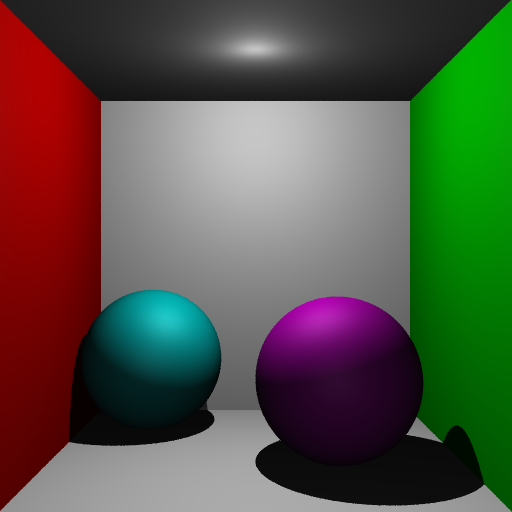
\includegraphics[width=\textwidth]{./img/perspective.png}
        \caption{透视投影}
    \end{subfigure}
    ~
    \begin{subfigure}{0.45\textwidth}
        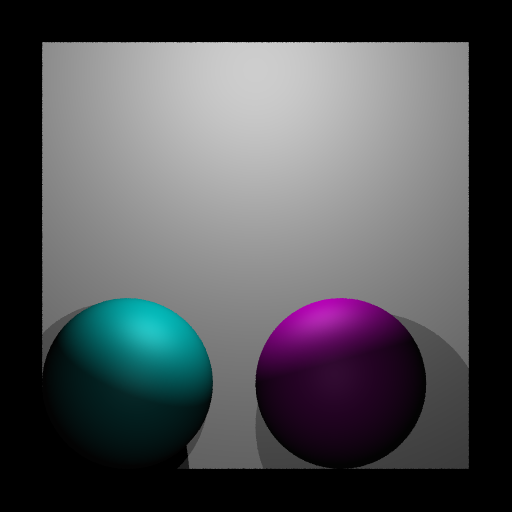
\includegraphics[width=\textwidth]{./img/ortho.png}
        \caption{正投影}
    \end{subfigure}
    \caption{不同投影效果对比}
    \label{fig:proj}
\end{figure}

\subsection {局部光照明}
在本次实验中使用Phong光照模型\footnote{\url{https://en.wikipedia.org/wiki/Phong_reflection_model}}对物体进行着色。对于物体上每个点局部光照的计算公式如下:
\[ I_{p}=k_{a}i_{a}+\sum_{m\in lights} (k_{d}(\hat{L_{m}}\cdot\hat{N})i_{m,d}+k_{s}(\hat{R_{m}}\cdot\hat{V})^{\alpha}i_{m,s}) \]

其中$k_{a},k_{d},k_{s},\alpha$为环境光反射系数、漫反射系数、高光系数、反光系数,$\hat{L_{m}},\hat{N},\hat{R_{m}},\hat{V}$分别为交点指向光源、交点处法向、入射光反射方向以及交点指向视点向量的归一化向量。

\subsection {阴影}
对于每个光线与物体的交点,需要从该点向所有光源发射阴影测试线,来判断该光源是否能照射到这一点。如果不能,则不计算该点的局部光照。
\subsubsection {软阴影}
为增加生成图像的真实感,考虑引入软阴影。通过在球面上均匀放置多个光强较小的点光源,从而达到模拟球体光源的效果。对比图见图\ref{fig:soft}。
\begin{figure}
    \centering
    \begin{subfigure}{0.45\textwidth}
        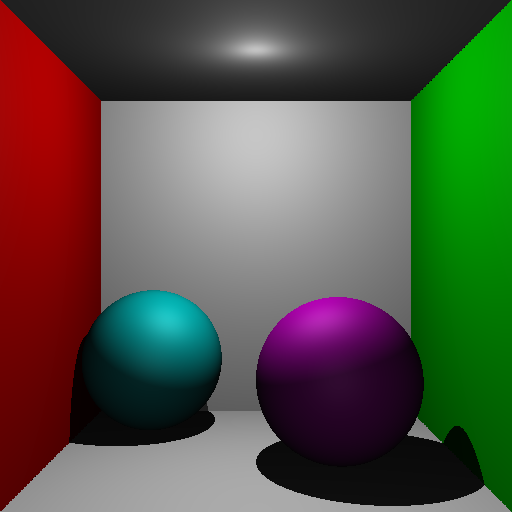
\includegraphics[width=\textwidth]{./img/without_soft.png}
        \caption{没有软阴影}
    \end{subfigure}
    ~
    \begin{subfigure}{0.45\textwidth}
        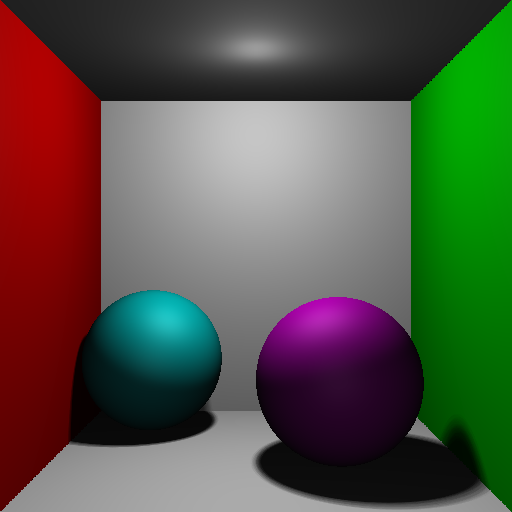
\includegraphics[width=\textwidth]{./img/soft.png}
        \caption{半径0.5,采样数10*10的软阴影效果}
    \end{subfigure}
    \caption{软阴影效果对比}
    \label{fig:soft}
\end{figure}

\subsection {物体的表示及求交}
\begin{description}[align=left,labelwidth=1.5cm]
\item[无限平面] 每个无限平面由一对法向及偏移量唯一构成。在判断交点位置时,首先判断光线是否与平面相交,之后通过计算光线起点在平面法线上的投影来得到结果。
\item[球] 每个球可以通过中心和半径来定义。可以通过上课讲过的几何法来判断光线与球的交点位置。
\item[三角形] 用三个顶点来定义三角形。采用了Moller-Trumbore方法\footnote{\url{http://pkuwwt.github.io/scholarship/2014-04-03-ray-triangle-intersection-tests-for-dummies/}} 来实现求交,该方法在得到交点的同时,也获取了交点同三个顶点的系数关系,为之后法向插值做准备。
\item[包围盒] 这里采用与坐标轴平行的包围盒。采用了Andrew Kensler方法\footnote{\url{http://psgraphics.blogspot.com/2016/02/new-simple-ray-box-test-from-andrew.html}} 进行求交,该方法使用了较少的计算和比较,主要是无需对NaN 情况进行特判,减少了一部分的计算量。
\end{description}

\subsection {光强衰减模型}
使用Lambert定律\footnote{\url{https://en.wikipedia.org/wiki/Beer–Lambert_law}}实现了对光强衰减的模拟计算,公式如下:
\[ I_{t}=I_{0}\cdot e^{-\tau}=I_{0}\cdot e^{-\mu l} \]
其中,$\mu$为衰减系数(实验中取为$0.02$),$l$为光线所走的距离。图\ref{fig:lambert}体现了有无光强衰减模型的区别。
\begin{figure}
    \centering
    \begin{subfigure}{0.4\textwidth}
        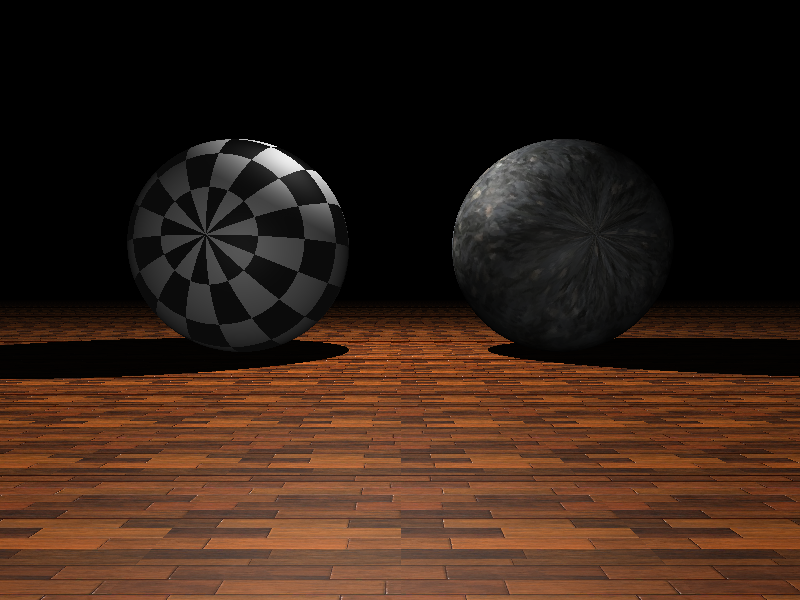
\includegraphics[width=\textwidth]{./img/without_lambert.png}
        \caption{没有衰减}
    \end{subfigure}
    ~
    \begin{subfigure}{0.4\textwidth}
        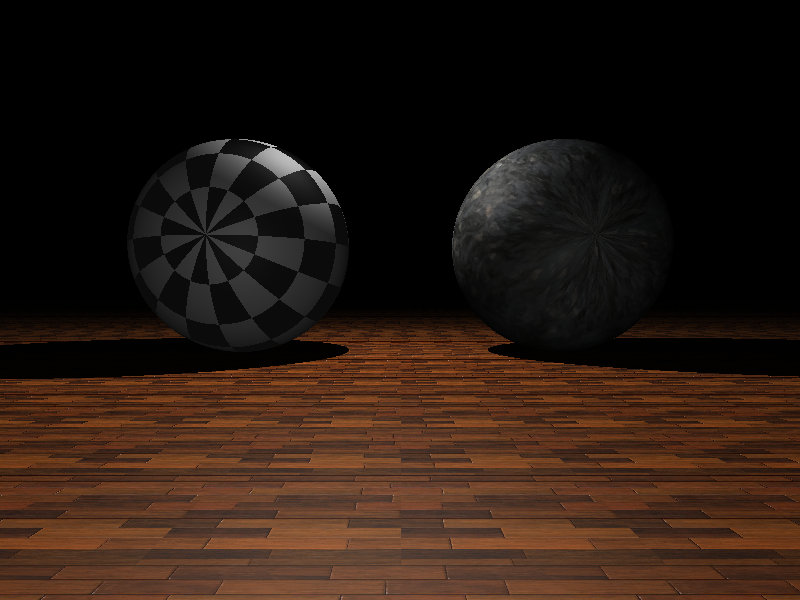
\includegraphics[width=\textwidth]{./img/lambert.png}
        \caption{存在衰减}
    \end{subfigure}
    \caption{光强衰减对比}
    \label{fig:lambert}
\end{figure}

\subsection {读入网格模型}
在本次实验中,读入网格模型(.obj文件)模块由自己完成,没有使用开源库。目前支持输入为三角网格的模型,且不支持纹理映射。在根目录下的"obj/"目录中存储的模型文件均可以被读取。

\subsection {纹理}
本次实验中实现了三种纹理:纯色纹理、黑白格纹理及图像纹理。对于纯色纹理,不存在纹理映射的问题;对其余两种纹理,需要对物体的纹理映射进行定义。

对无限平面来说,首先计算出该平面的一组相互垂直的单位向量。那么对平面上任何一点,可以算出它相对这对单位向量的二维坐标,从而实现从三维点到二维坐标的映射。

对球上任意一点,可以将其转换为球面坐标。由于球面参数方程仅具有两个参数,所以对该方程反求出这两个参数,就可以得到纹理映射。

由于网格模型结构比较复杂,故没有实现在网格模型上的黑白格及图像纹理,仅支持纯色纹理。

\subsection {KD树}
本实验中采用了基于SAH的KD树构建,构建算法参考了\cite{wald2006building}的快速构建SAH-KD树算法,将建树算法的时间复杂度降低至$O(NlogN)$。基于表面积启发式的KD 树在查询操作上与基于中值切割的KD树相比,效率提高了许多,这主要是由于基于SAH的建树方法倾向于选择切分后遍历代价较小的切分平面,而不只是简单地选取包围盒中心的中值进行切分。

构建这种KD树时需要考虑两个参数:叶结点内最多管理物体的个数及KD树的深度。针对只有龙模型的场景进行建树并且渲染的测试,建树与渲染均为单线程,测试数据如表\ref{table:kdtree_manage},可以看出建树时间与渲染时间存在一个权衡。\\
\begin{table}
    \centering
    \begin{tabular}{l c c}
    Time/s & build & render\\
    \hline
    100层\ 5个 & 1.56 & 2.90\\
    100层\ 10个 & 1.51 & 2.96\\
    100层\ 20个 & 1.31 & 3.21\\
    \end{tabular}
    \caption{}
    \label{table:kdtree_manage}
\end{table}

\subsubsection {遍历方法}
对于KD树中每个内部结点,存放着一个分割平面$P$,结点的左、右儿子分别管理与左、右空间有交集(与$P$重合的物体作为特殊情况在\cite{wald2006building}中有说明)的那一部分物体。光线与结点求交的过程可以分为如下几步:首先与分割出的左、右空间进行求交,如果仅与其中一个空间有交,则只遍历那个空间;否则先遍历光线首先遍历到的空间,后遍历另外那半个空间。这样可以保证不漏掉任何物体,且不遍历明显没有交点的情况。
\par 在本次实验中采用递归的方法对遍历进行实现。我尝试了将其改为非递归方法,但发现经过编译器优化后,表现反而不如递归方法,故仍采用原方法。

\subsection {光滑着色}
双线性法向插值方法进行光滑着色。首先对模型中顶点计算其相邻网格面的法向平均值,作为其法向,随后对网格面上任意一点,可以通过该面上三个顶点的法向插值得到该点的法向,在该点作为光线与物体的交点时,就可以使用该法向值进行局部光照的计算。对于犹他茶壶的对比图见图\ref{fig:smooth},可以看出壶身和壶嘴部分的差距比较明显。
\begin{figure}
    \centering
    \begin{subfigure}{0.45\textwidth}
        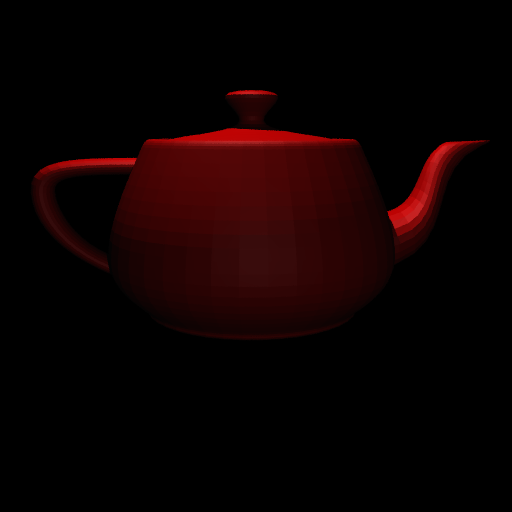
\includegraphics[width=\textwidth]{./img/without_smooth.png}
        \caption{不光滑着色}
    \end{subfigure}
    ~
    \begin{subfigure}{0.45\textwidth}
        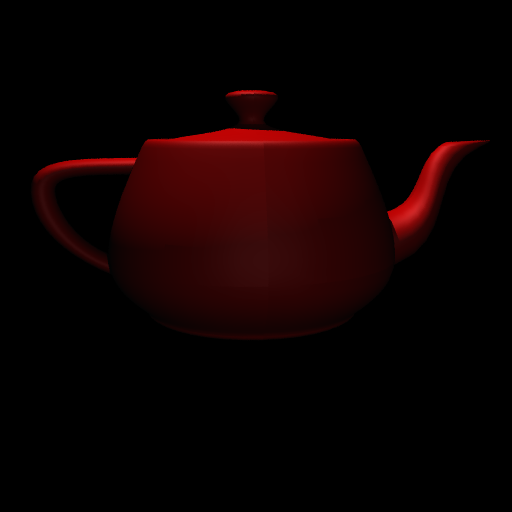
\includegraphics[width=\textwidth]{./img/smooth.png}
        \caption{光滑着色}
    \end{subfigure}
    \caption{光滑着色对比}
    \label{fig:smooth}
\end{figure}

\subsection {抗锯齿}
采用抖动采样法进行抗锯齿处理。之前只是将虚拟屏幕中每个像素对应的小方格的中央点看做追踪光线所指的方向,现在需要多次在小方格中随机采样,分别追踪之,得到所有颜色值后取平均,也就近似获得了该像素的正确颜色值。
\begin{figure}
    \centering
    \begin{subfigure}{\textwidth}
        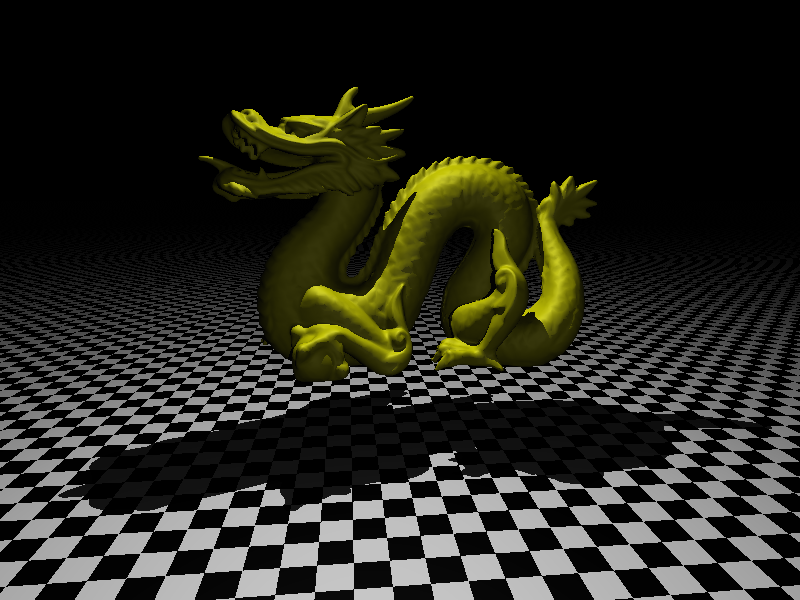
\includegraphics[width=\textwidth]{./img/without_anti.png}
        \caption{没有抗锯齿}
    \end{subfigure}
    \begin{subfigure}{\textwidth}
        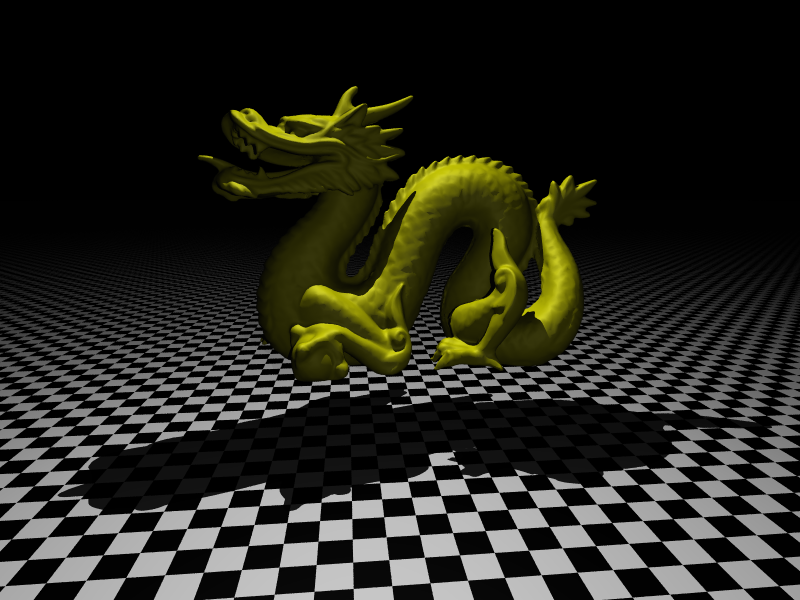
\includegraphics[width=\textwidth]{./img/anti.png}
        \caption{抗锯齿}
    \end{subfigure}
    \caption{抗锯齿对比}
    \label{fig:anti}
\end{figure}

根据图\ref{fig:anti}可以从地板纹理及龙模型的细节看出有无抗锯齿的差别。在没有抗锯齿的情况下,地面的黑白格纹理在远方变形得十分严重,这个问题在经过抗锯齿操作后得到了解决。

\subsection {景深}
根据照相机的参数,可以模拟景深效果,也即在焦平面附近的景物可以显示得较为清楚,过近或过远都会产生一定模糊的现象。对于虚拟屏幕中的某个像素,位置为$P$,视点中心位置为$O$,连接$OP$ 并延长,求出其与焦平面的交点$T$。之后在光圈内随机采样一些点$A_{i}$,需要追踪的光线即为$\overrightarrow{A_{i}T}$。根据图\ref{fig:dop} 可以看出加入景深效果后的渲染效果相较前者要真实许多。
\begin{figure}
    \centering
    \begin{subfigure}{0.45\textwidth}
        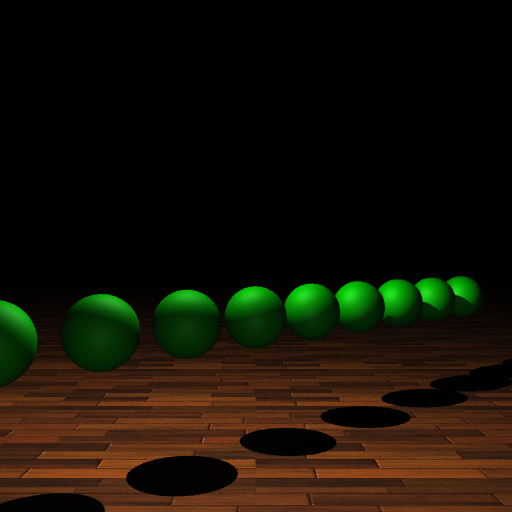
\includegraphics[width=\textwidth]{./img/without_dop.png}
        \caption{无景深}
    \end{subfigure}
    ~
    \begin{subfigure}{0.45\textwidth}
        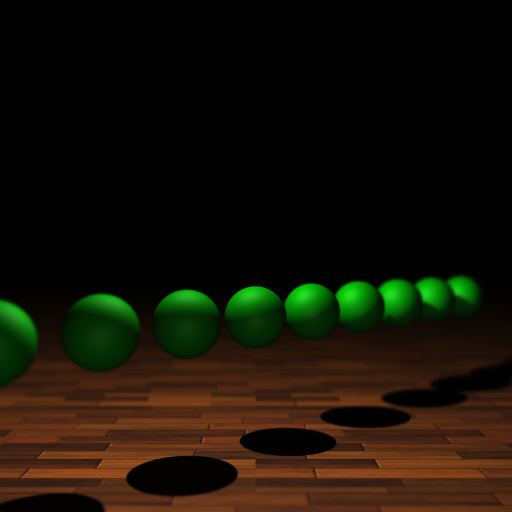
\includegraphics[width=\textwidth]{./img/dop.png}
        \caption{采样数30的景深效果}
    \end{subfigure}
    \caption{景深效果对比}
    \label{fig:dop}
\end{figure}

\subsection {并行加速}
本实验中在建KD树及追踪光线这两处进行了CPU多线程加速,均使用VS2013所支持的openmp2.0实现。
\subsubsection {建KD树}
由于建树是一个递归过程,对每个结点会递归对它的左、右孩子递归进行建树操作。在实现时,首先获取执行计算机CPU的核数,随后每次进行递归建树操作时,如果分配给当前函数的核数大于1,则将核数平分给左、右两个建树过程;否则不采用多线程加速。

针对只有一个网格模型的场景进行KD树的建树测试,测试数据如表\ref{table:parallel_build},可以发现并行后的效率提高了约六成。\\
\begin{table}
    \centering
    \begin{tabular}{l c c c}
    Build time/ms & teapot & bunny & dragon\\
    \hline
    Before parallelization & 78 & 108 & 1507\\
    After parallelization & 48 & 69 & 948\\
    \end{tabular}
    \caption{}
    \label{table:parallel_build}
\end{table}
\subsubsection {追踪光线}
由于每个计算每个像素的颜色是独立的,可以使用openmp对for循环进行自动并行处理。这里如果直接使用openmp并行化,由于不同像素计算复杂度不同,可能会出现不同线程完成速度不同,从而导致资源的浪费。我采用的办法是对纵、横两个维度($0\rightarrow width,0\rightarrow height$)分别进行随机排列,再进行并行计算,这样就会在一定程度上减少资源的浪费情况,而且随机排列过程也不会占用太多时间。
\par 针对只有一个网格模型的场景进行渲染测试,测试数据如表\ref{table:parallel_trace},可以发现并行后的效率约是单线程的3倍。\\
\begin{table}
    \centering
    \begin{tabular}{l c c c}
    Render time/s & teapot & bunny & dragon\\
    \hline
    Before parallelization & 1.28 & 1.52 & 3.04\\
    After parallelization & 0.37 & 0.46 & 0.94\\
    \end{tabular}
    \caption{}
    \label{table:parallel_trace}
\end{table}
